%%%%%%%%%%%%%%%%%%%%%%%%%%%%%%%%%%%%%%%%%
% Beamer Presentation
% LaTeX Template
% Version 2.0 (March 8, 2022)
%
% This template originates from:
% https://www.LaTeXTemplates.com
%
% Author:
% Vel (vel@latextemplates.com)
%
% License:
% CC BY-NC-SA 4.0 (https://creativecommons.org/licenses/by-nc-sa/4.0/)
%
%%%%%%%%%%%%%%%%%%%%%%%%%%%%%%%%%%%%%%%%%

%----------------------------------------------------------------------------------------
%	PACKAGES AND OTHER DOCUMENT CONFIGURATIONS
%----------------------------------------------------------------------------------------

\documentclass[
	10pt, % Set the default font size, options include: 8pt, 9pt, 10pt, 11pt, 12pt, 14pt, 17pt, 20pt
	%t, % Uncomment to vertically align all slide content to the top of the slide, rather than the default centered
	aspectratio=169, % Uncomment to set the aspect ratio to a 16:9 ratio which matches the aspect ratio of 1080p and 4K screens and projectors
]{beamer}

\usepackage[all]{xy}

\usepackage[spanish]{babel}
\usepackage[utf8]{inputenc}

\graphicspath{{Images/}{./}} % Specifies where to look for included images (trailing slash required)

\usepackage{booktabs} % Allows the use of \toprule, \midrule and \bottomrule for better rules in tables

%\usepackage{tikz}
%\usetikzlibrary{positioning}
%\usetikzlibrary{shapes,arrows,arrows,positioning,fit}

\usepackage{tikz}
\usetikzlibrary{mindmap}
\usetikzlibrary{arrows, positioning}
\usetikzlibrary{arrows, shapes, positioning, shadows, trees}

\usepackage{forest}

\usepackage{multirow}

\usepackage{graphicx}
\usepackage{hyperref}

\usepackage{xcolor,listings}
\usepackage{textcomp}
%\usepackage{color}

\usepackage{enumitem}

\usepackage{xcolor}

\usepackage{verbatim}

\providecommand{\abs}[1]{\lvert#1\rvert}

%----------------------------------------------------------------------------------------
%	SELECT LAYOUT THEME
%----------------------------------------------------------------------------------------

% Beamer comes with a number of default layout themes which change the colors and layouts of slides. Below is a list of all themes available, uncomment each in turn to see what they look like.

%\usetheme{default}
%\usetheme{AnnArbor}
%\usetheme{Antibes}
%\usetheme{Bergen}
%\usetheme{Berkeley}
%\usetheme{Berlin}
%\usetheme{Boadilla} % interesante
%\usetheme{CambridgeUS}
%\usetheme{Copenhagen}
%\usetheme{Darmstadt}
%\usetheme{Dresden}
%\usetheme{Frankfurt}
%\usetheme{Goettingen}
%\usetheme{Hannover}
%\usetheme{Ilmenau}
%\usetheme{JuanLesPins}
%\usetheme{Luebeck}
\usetheme{Madrid} % interesante
%\usetheme{Malmoe}
%\usetheme{Marburg}
%\usetheme{Montpellier}
%\usetheme{PaloAlto}
%\usetheme{Pittsburgh} % interesante
%\usetheme{Rochester} % interesante este
%\usetheme{Singapore}
%\usetheme{Szeged}
%\usetheme{Warsaw}

%----------------------------------------------------------------------------------------
%	SELECT COLOR THEME
%----------------------------------------------------------------------------------------

% Beamer comes with a number of color themes that can be applied to any layout theme to change its colors. Uncomment each of these in turn to see how they change the colors of your selected layout theme.

%\usecolortheme{albatross}
%\usecolortheme{beaver}
%\usecolortheme{beetle}
%\usecolortheme{crane}
%\usecolortheme{dolphin}
%\usecolortheme{dove}
%\usecolortheme{fly}
%\usecolortheme{lily}
%\usecolortheme{monarca}
%\usecolortheme{seagull}
%\usecolortheme{seahorse}
\usecolortheme{spruce} % verde suave
%\usecolortheme{whale}
%\usecolortheme{wolverine}

%----------------------------------------------------------------------------------------
%	SELECT FONT THEME & FONTS
%----------------------------------------------------------------------------------------

% Beamer comes with several font themes to easily change the fonts used in various parts of the presentation. Review the comments beside each one to decide if you would like to use it. Note that additional options can be specified for several of these font themes, consult the beamer documentation for more information.

\usefonttheme{default} % Typeset using the default sans serif font
%\usefonttheme{serif} % Typeset using the default serif font (make sure a sans font isn't being set as the default font if you use this option!)
%\usefonttheme{structurebold} % Typeset important structure text (titles, headlines, footlines, sidebar, etc) in bold
%\usefonttheme{structureitalicserif} % Typeset important structure text (titles, headlines, footlines, sidebar, etc) in italic serif
%\usefonttheme{structuresmallcapsserif} % Typeset important structure text (titles, headlines, footlines, sidebar, etc) in small caps serif

%------------------------------------------------

%\usepackage{mathptmx} % Use the Times font for serif text
%\usepackage{palatino} % Use the Palatino font for serif text

\usepackage{helvet} % Use the Helvetica font for sans serif text
%\usepackage[default]{opensans} % Use the Open Sans font for sans serif text
%\usepackage[default]{FiraSans} % Use the Fira Sans font for sans serif text
\usepackage[default]{lato} % Use the Lato font for sans serif text

%----------------------------------------------------------------------------------------
%	SELECT INNER THEME
%----------------------------------------------------------------------------------------

% Inner themes change the styling of internal slide elements, for example: bullet points, blocks, bibliography entries, title pages, theorems, etc. Uncomment each theme in turn to see what changes it makes to your presentation.

%\useinnertheme{default}
\useinnertheme{circles}
%\useinnertheme{rectangles}
%\useinnertheme{rounded}
%\useinnertheme{inmargin}

%----------------------------------------------------------------------------------------
%	SELECT OUTER THEME
%----------------------------------------------------------------------------------------

% Outer themes change the overall layout of slides, such as: header and footer lines, sidebars and slide titles. Uncomment each theme in turn to see what changes it makes to your presentation.

%\useoutertheme{default}
%\useoutertheme{infolines}
%\useoutertheme{miniframes}
%\useoutertheme{smoothbars}
%\useoutertheme{sidebar}
%\useoutertheme{split}
%\useoutertheme{shadow}
%\useoutertheme{tree}
%\useoutertheme{smoothtree}

\setbeamertemplate{footline} % Uncomment this line to remove the footer line in all slides
%\setbeamertemplate{footline}[page number] % Uncomment this line to replace the footer line in all slides with a simple slide count

\setbeamertemplate{navigation symbols}{} % Uncomment this line to remove the navigation symbols from the bottom of all slides

%----------------------------------------------------------------------------------------
%	PRESENTATION INFORMATION
%----------------------------------------------------------------------------------------

\title[Short Title]{Sistemas de Recuperación de Información} % The short title in the optional parameter appears at the bottom of every slide, the full title in the main parameter is only on the title page

\subtitle{Introducción a los SRI} % Presentation subtitle, remove this command if a subtitle isn't required

\author{Lic. Carlos León González \\ Dra.C. Lucina García Hernández} % Presenter name(s), the optional parameter can contain a shortened version to appear on the bottom of every slide, while the main parameter will appear on the title slide

\institute[UC]{Facultad de Matem\'atica y Computaci\'on \\ Universidad de La Habana \\ \smallskip } % Your institution, the optional parameter can be used for the institution shorthand and will appear on the bottom of every slide after author names, while the required parameter is used on the title slide and can include your email address or additional information on separate lines

\date{22 de enero de  2024} % Presentation date or conference/meeting name, the optional parameter can contain a shortened version to appear on the bottom of every slide, while the required parameter value is output to the title slide

%----------------------------------------------------------------------------------------

\begin{document}

\lstset{
	literate=%
	{á}{{\'a}}1
	{í}{{\'i}}1
	{é}{{\'e}}1
	{ý}{{\'y}}1
	{ú}{{\'u}}1
	{ó}{{\'o}}1
	{ě}{{\v{e}}}1
	{š}{{\v{s}}}1
	{č}{{\v{c}}}1
	{ř}{{\v{r}}}1
	{ž}{{\v{z}}}1
	{ď}{{\v{d}}}1
	{ť}{{\v{t}}}1
	{ň}{{\v{n}}}1                
	{ů}{{\r{u}}}1
	{Á}{{\'A}}1
	{Í}{{\'I}}1
	{É}{{\'E}}1
	{Ý}{{\'Y}}1
	{Ú}{{\'U}}1
	{Ó}{{\'O}}1
	{Ě}{{\v{E}}}1
	{Š}{{\v{S}}}1
	{Č}{{\v{C}}}1
	{Ř}{{\v{R}}}1
	{Ž}{{\v{Z}}}1
	{Ď}{{\v{D}}}1
	{Ť}{{\v{T}}}1
	{Ň}{{\v{N}}}1                
	{Ů}{{\r{U}}}1    
}

%----------------------------------------------------------------------------------------
%	TITLE SLIDE
%----------------------------------------------------------------------------------------

\begin{frame}
	\titlepage % Output the title slide, automatically created using the text entered in the PRESENTATION INFORMATION block above
	
	\centering
	\url{https://t.me/matcom_sri_2024}
\end{frame}

%------------------------------------------------
% Motivación

\begin{frame}
	
	\frametitle{Cada minuto de Internet en 2023}
	
	\centering
	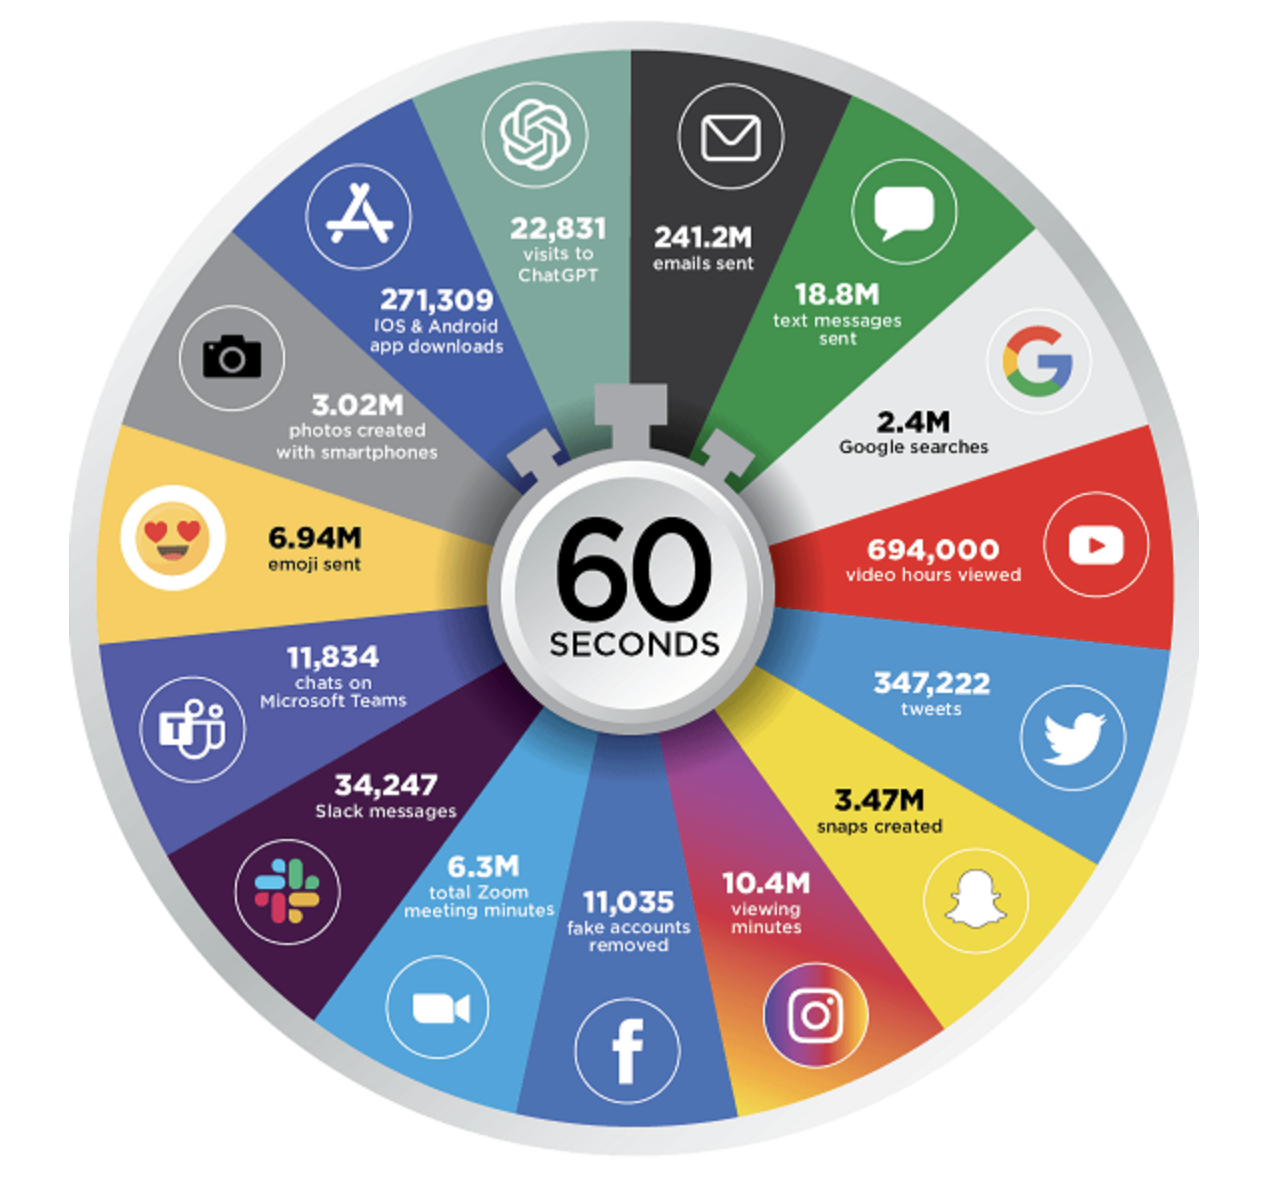
\includegraphics[scale=0.36]{info-2023.png} 
	
	{\scriptsize Tomado de https://ediscoverytoday.com/2023/04/20/2023-internet-minute-infographic-by-ediscovery-today-and-ltmg-ediscovery-trends/}
	
\end{frame}

%------------------------------------------------
% Motivación

\begin{frame}
	
	\frametitle{Cada minuto de Internet en 2023}
	
	\noindent\begin{minipage}{.4\textwidth}
		
		\visible<1->{\textcolor{purple}{¿Toda la información puede almacenarse en una base de datos relacional?}} \\
		
		\visible<2->{\textcolor{purple}{Entonces, ¿dónde y cómo puede almacenarse la información?}} \\
		
		\visible<3->{\textcolor{purple}{¿Cómo el sistema es capaz, de forma automática, detectar ``nueva'' información?}} \\
		
		\visible<4->{\textcolor{purple}{¿Cómo se inserta esa información en la ``base de datos'' para que sea coherente con la realidad?}} \\
		
		\visible<5->{\textcolor{purple}{¿Cómo recuperar la información requerida, si la consulta es definida en lenguaje natural?}}
		
	\end{minipage}%
	\begin{minipage}{.7\textwidth}
		\centering
		\includegraphics<1->[scale=0.36]{info-2023.png} 
	\end{minipage}
	
	\centering
	
\end{frame}

%------------------------------------------------
%Objetivos de la asignatura 

\begin{frame}
	
	\frametitle{Objetivos de la asignatura}
	
	\begin{itemize}
		
		\item Asimilar las características de los Sistemas de Información, su modelación matemática-computacional y su desarrollo e implementación.
		
		\item Asimilar y desarrollar herramientas para la búsqueda, extracción, almacenamiento y recuperación de información.
		
		\item Aplicar la modelación matemática al análisis y evaluación de los sistemas y fuentes de información.
		
	\end{itemize}
	
	
	
\end{frame}

%------------------------------------------------
% ¿Qué es un Sistema de Recuperación de Información?

\begin{frame}
	
	\frametitle{¿Qué es un Sistema de Recuperación de Información?}
	
	\begin{alertblock}{} 
		La \textbf{Recuperación de Información} es la localización de materiales (generalmente documentos) de naturaleza no estructurada (generalmente texto) para satisfacer una necesidad de información en una larga colección (generalmente almacenada en computadoras).
		
		\raggedleft{\textcolor{gray}{Manning, C. D., “Introduction to Information Retrieval”, Cap. 1, pág. 1}}
	\end{alertblock}
	
	\vspace{2\baselineskip}
	
	\pause
	Luego, aquellos sistemas que implementan la recuperación de información para obtener documentos, registros, imágenes, sonidos, etc., e interaccionan con usuarios o servicios que requieren obtener información, son conocidos como \textbf{Sistemas de Recuperación de Información}.
	
\end{frame}

%------------------------------------------------
%Evolución

\begin{frame}[fragile]
	
	\frametitle{Evolución}
	
	\centering
	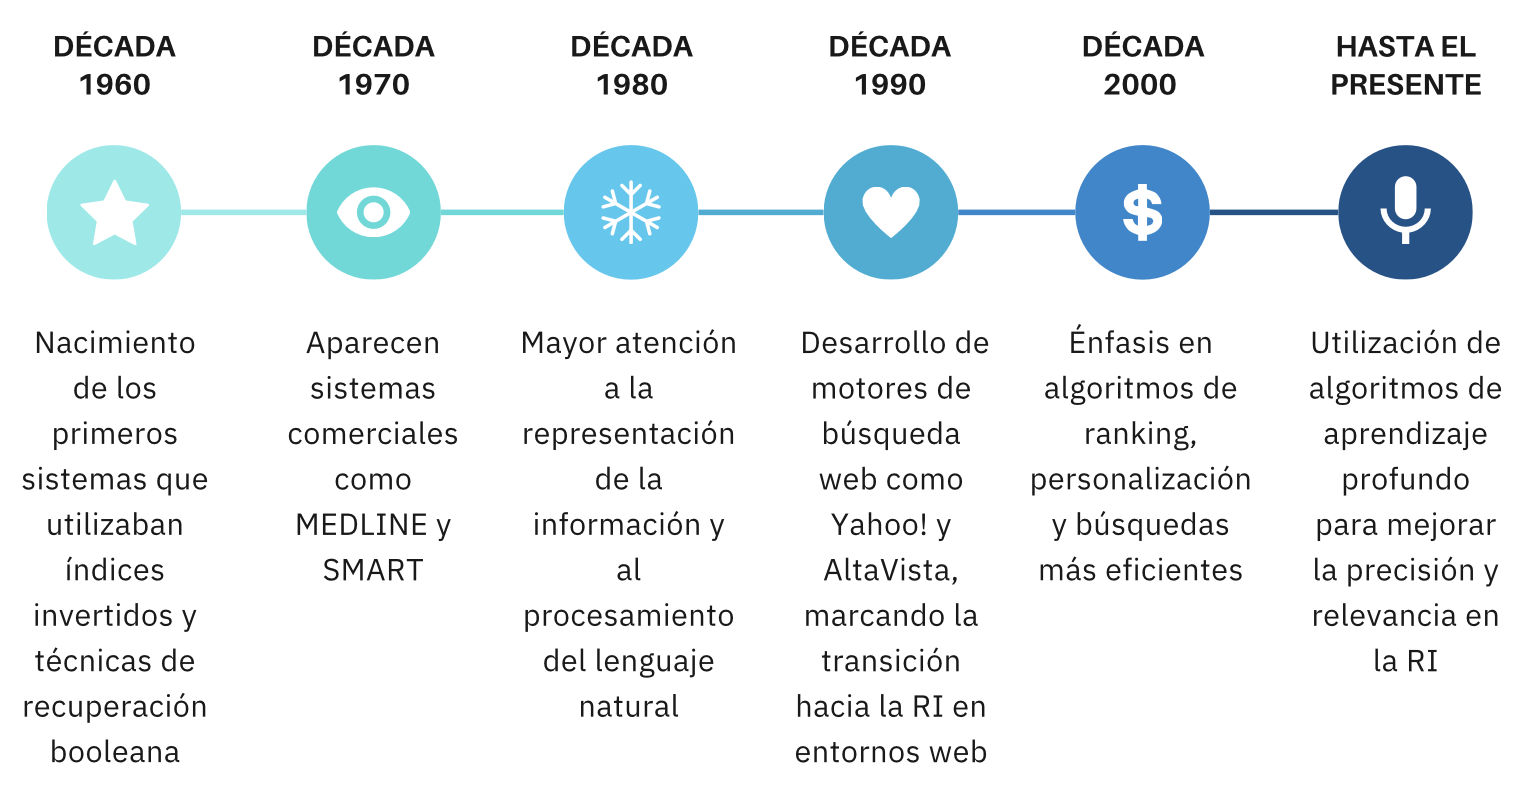
\includegraphics[scale=0.55]{evolucion.png} 
	
\end{frame}

%------------------------------------------------
% Definición formal

\begin{frame}[fragile]
	
	\frametitle{Definición formal}
	
	\begin{alertblock}{} 
		Un \textbf{modelo de recuperación de información} es un cuádruplo $[D, Q, F, R(q_j, d_j)]$ donde:  
		
		\vspace{1\baselineskip}
		\textbf{D} es un conjunto de representaciones lógicas de los datos de la colección.
		
		\vspace{1\baselineskip}
		\textbf{Q} es un conjunto compuesto por representaciones lógicas de las necesidades del usuario, denominadas ``consultas''.
		
		\vspace{1\baselineskip}
		\textbf{F} es un framework para modelar las representaciones de los datos, consultas y sus relaciones.
		
		\vspace{1\baselineskip}
		\textbf{R} es una función de ranking que asocia un número real a una consulta $q \in Q$ y un documento $d \in D$. La evaluación de esta función establece un cierto orden entre la información de acuerdo a la consulta.
	
	\end{alertblock}
	
\end{frame}

%------------------------------------------------
% Estructura de un SRI

\begin{frame}
	
	\frametitle{Estructura de un SRI}
	
	\centering
	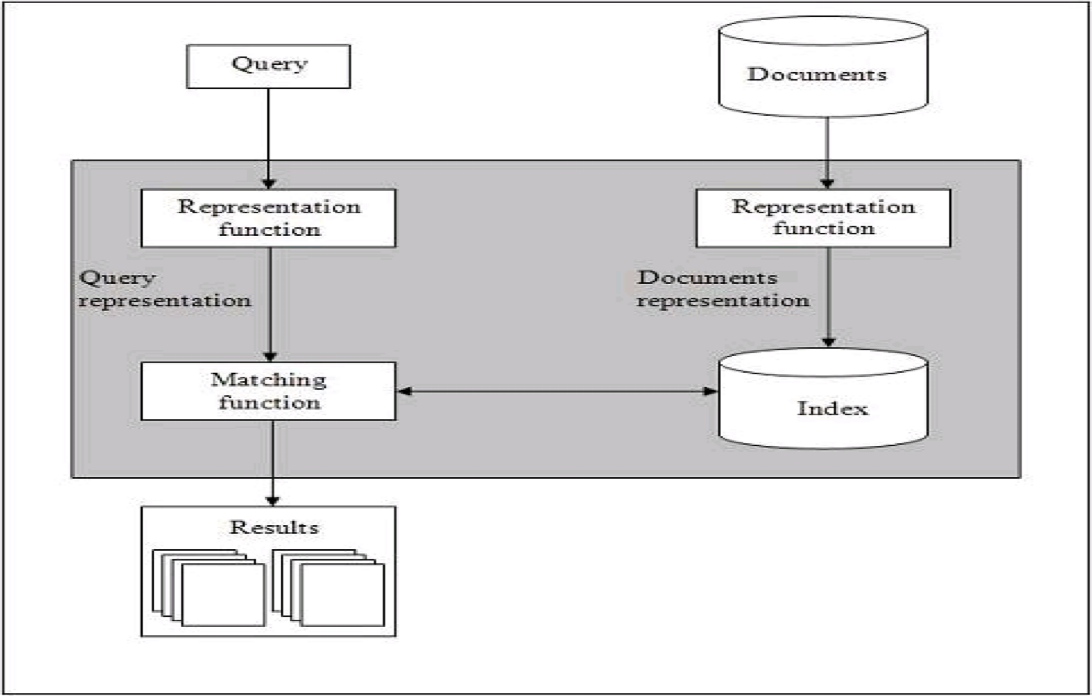
\includegraphics[scale=0.6]{sistema_basico.png} 
	
	{\scriptsize Tomado de https://www.analyticsvidhya.com/blog/2021/06/part-20-step-by-step-guide-to-master-nlp-information-retrieval/}
	
\end{frame}

%------------------------------------------------
% Tipos básicos de SRI

\begin{frame}
	
	\frametitle{Tipos básicos de SRI}
	
	\centering
	\begin{forest}
		for tree={grow'=east, anchor=west}
		[ Modelo de RI, 
			[
				Clásico, 
				for children={tier=1} 
				[
					Booleano, 
					for children={tier=2} 
						[Difuso]
						[Extendido]
				]
				[
					Vectorial, 
					for children={tier=2} 
						[Vector Generalizado]
						[Semántica Latente]
						[Redes Neuronales]
				]
				[
				Probabilístico, 
				for children={tier=2} 
					[Redes de Inferencia]
					[Redes de Creencia]
				]
			] 
			[
				Estructurado, 
				for children={tier=1}
					[Listas no Solapadas]
					[Nodos Proximales]
			]
		]
	\end{forest}

\end{frame}

%------------------------------------------------
% Modelo vectorial. Introducción

\begin{frame}
	
	\frametitle{Modelo Vectorial. Introducción}
	
	Modelo basado en el Álgebra Vectorial.
	
	\vspace{1\baselineskip}
	
	Los modelos tradicionales de recuperación de información asumen que cada documento se representa mediante un conjunto de palabras clave, conocidas como términos indexados. 
	
	\vspace{1\baselineskip}
	
	\pause
	Estos términos capturan la esencia temática del documento y se emplean para indexar, caracterizar y resumir el contenido del documento. 
	
	\vspace{1\baselineskip}
	Los términos indexados se centran principalmente en sustantivos, pero no necesariamente y no todos tienen la misma relevancia para describir un documento.
	
	\pause
	\vspace{1\baselineskip}
	\begin{alertblock}{} 
		El peso para todo par ($k_i, d_j$), donde $k_i$ es el $i$-ésimo término indexado y $d_j$ el $j$-ésimo documento, se define como $w_{i,j} \geq 0$. La consulta es considerada como un documento durante el análisis y se representa como $q$. Luego, cada documento es representado como $\vec{d_j} = (w_{1, j}, \dots, w_{t, j})$.
	\end{alertblock}
	
\end{frame}

%------------------------------------------------
% Modelo vectorial. Función de similitud

\begin{frame}
	
	\frametitle{Modelo vectorial. Función de similitud}
	
	Función conocida como \textbf{distancia coseno}.
	
	\centering
	$$
		sim(\vec{d_j}, \vec{q}) 
		= \frac{ \vec{d_j} \bullet \vec{q}}{ \abs{\vec{d_j}} \times \abs{\vec{q}}}
		= \frac{\sum_{i=1}^{t} w_{i, j} \times w_{i, q}}{\sqrt{\sum_{i=1}^{t} w_{i, j}^2} \times \sqrt{\sum_{i=1}^{t} w_{i, q}^2}} 
	$$
	
	$$sim(\vec{d_j}, \vec{q}) \in [0; 1]$$
	
	\end{frame}

%------------------------------------------------
% Modelo vectorial. Cálculo del peso del término

\begin{frame}
	
	\frametitle{Modelo vectorial. Cálculo del peso del término}
	
	\begin{itemize}
		
		\item Frecuencia del término  
		$$tf_{i, j} = \frac{freq_{i,j}}{max_l freq_{l, j}}$$
		donde \\
		\hspace*{4mm} $freq_{i,j}$ representa la frecuencia del término $i$ en el documento $j$ \\
		\hspace*{4mm} $max_l freq_{l, j}$ representa la mayor frecuencia de los términos del documento $j$ 
		
		\pause
		\item Frecuencia inversa del documento 
		$$idf_i = \log(\frac{N}{n_i})$$
		donde \\ 
		\hspace*{4mm} $N$ representa la cantidad de documentos del corpus \\
		\hspace*{4mm} $n_i$ representa la cantidad de documentos en los cuales aparece el término $k_i$
		
	\end{itemize}
	
	\pause
	Luego, 
	$$w_{i,j} = tf_{i, j} \times idf_i =(\alpha + (1 - \alpha) \frac{freq_{i,j}}{max_l freq_{l, j}}) \times \log(\frac{N}{n_i}) $$
	con $\alpha \in [0, 1]$
	
\end{frame}

%------------------------------------------------
% Modelo vectorial. Definición

\begin{frame}
	
	\frametitle{Modelo vectorial. Definición}
		
	\vspace{1\baselineskip}
	\textbf{D} 
	\only<1>{Conjunto de representaciones lógicas de los datos de la colección}
	\only<2->{Vectores de los pesos asociados a los términos de los documentos (no binarios)}
	
	\vspace{1\baselineskip}
	\textbf{Q} 
	\only<1-2>{Conjunto compuesto por representaciones lógicas de las necesidades del usuario, denominadas ``consultas''}
	\only<3->{Vectores de los pesos asociados a los términos de los documentos (no binarios)}
	
	\vspace{1\baselineskip}
	\textbf{F} 
	\only<1-3>{Framework para modelar las representaciones de los datos, consultas y sus relaciones}
	\only<4->{Espacio $n$-dimensional y operaciones del álgebra lineal entre vectores}
	
	\vspace{1\baselineskip}
	\textbf{R} 
	\only<1-4>{Función de ranking}
	\only<5->{$sim(d_j, q) = \frac{\sum_{i=1}^{t} w_{i, j} \times w_{i, q}}{\sqrt{\sum_{i=1}^{t} w_{i, j}^2} \times \sqrt{\sum_{i=1}^{t} w_{i, q}^2}} $}
	
	
	
\end{frame}

%------------------------------------------------
% Sistema de evaluación

\begin{frame}[fragile]
		
	\frametitle{Sistema de evaluación}
	
	\noindent\begin{minipage}{.4\textwidth}
		\centering
		\begin{itemize}
			\item<1-> Trabajo de control
			\begin{itemize}
				\item Penúltima semana del curso
			\end{itemize}
			
			\item<2-> Proyecto acumulativo
			\begin{itemize}
				\item Implementación de módulos durante los laboratorios
				\item A desarrollar en equipos de \textbf{2 personas}
				\item Revisión: segunda semana posterior al último contenido impartido referente
			\end{itemize}
			
			\item<3-> Proyecto
			\begin{itemize}
				\item A desarrollar en equipos de \textbf{2 personas}
				\item Revisión: última semana del curso o cuando los estudiantes culminen
			\end{itemize}
		\end{itemize}
		
	\end{minipage}%
	\begin{minipage}{.7\textwidth}
		\centering
		\includegraphics<1->[scale=1]{nina-llorando.jpeg} 
	\end{minipage}

	
	
	
\end{frame}

%------------------------------------------------
% Dudas

\begin{frame}
	
	\frametitle{Dudas, preguntas, sugerencias ...}
	
	\begin{figure}[h]
		\centering
		
\includegraphics[scale=0.38]{duda_1.jpg}
	\end{figure}
	
\end{frame}

%------------------------------------------------
% Objetivos de la clase

\begin{frame}
	
	\frametitle{Ideas esenciales abordadas en la clase}
	
	\begin{itemize}
		
		\item Definición de RI y SRI
		
		\item Tipos de SRI
		
		\item Definición del Modelo Vectorial
		
		\item Sistema evaluativo del curso
		
	\end{itemize}
	
	
	
\end{frame}

%------------------------------------------------
% Bibliografía

\begin{frame}
	
	\frametitle{Bibliografía}
	
	\begin{itemize}
		\item Baeza-Yates, R., Ribeiro-Neto, B (2002) Modern Information Retrieval.
		
		\item Manning, C. D. (2009). An Introduction to Information Retrieval . Cambridge UP
		
		\item Baeza-Yates, R. a. (s.f.). Information Retrieval: Data Structures \& Algorithms. 
	\end{itemize}
	
\end{frame}

%------------------------------------------------

\begin{frame}
	\titlepage
\end{frame}



\end{document} 